\documentclass[9pt]{article}

\usepackage{amsmath}
\usepackage{tcolorbox}
% `parskip` removes indentation for all paragraphs: http://tex.stackexchange.com/a/55016
\usepackage{parskip}
% Allows us to color rows / cols of a table.
% See https://texblog.org/2011/04/19/highlight-table-rowscolumns-with-color/
\usepackage{color, colortbl}

\usepackage{graphicx}
\graphicspath{{images/ps2a/}}

\usepackage{hyperref}

\leftmargin=0.25in
\oddsidemargin=0.25in
\textwidth=6.0in
\topmargin=-0.25in
\textheight=9.25in

\definecolor{Gray}{gray}{0.9}

\begin{document}

\begin{center}
  \large\textbf{MIT 18.01 Problem Set 2A Unofficial Solutions}
\end{center}

\begin{tcolorbox}
  \textbf{Q1)} Graph the even and odd functions you found in Problem 1, Part II of PS1. Directly below, graph their derivatives. Do this qualitatively using your estimation of the slope. Do not use the formulas for the derivatives (except to check your work if you want). You can use a graphing calculator to check your answer, provided that you mention it in Problem 0. (Note, however, that you may not use books, notes or calculators during tests, so it is unwise to rely on a graphing calculator here.)
\end{tcolorbox}

\begin{align*}
  \frac{x - 1}{x + 1} &= \frac{x - 1}{x + 1} \cdot \frac{x - 1}{x - 1}\\
                      &= \frac{x^2 - 2x + 1}{x^2 - 1}\\
                      &= \frac{x^2 + 1}{x^2 - 1} - \frac{2x}{x^2 - 1}
\end{align*}

so the even function is $\frac{x^2 + 1}{x^2 - 1}$ and the odd function is $-\frac{2x}{x^2 - 1}$

\begin{center}
  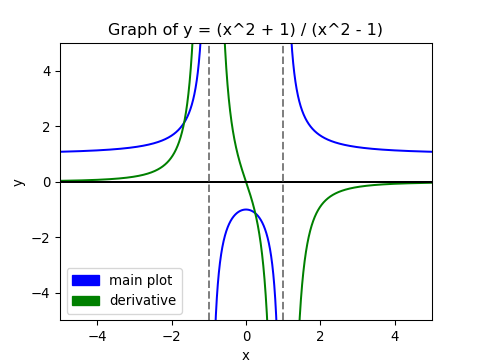
\includegraphics[scale=0.8]{q1_even.png}
\end{center}

\begin{center}
  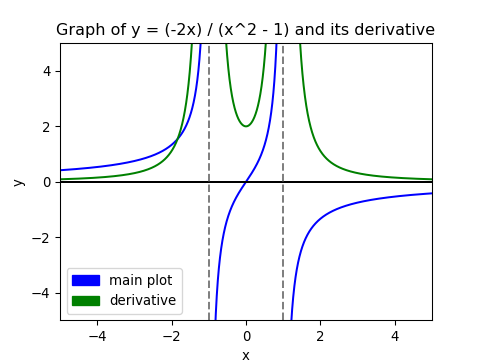
\includegraphics[scale=0.8]{q1_odd.png}
\end{center}


\begin{tcolorbox}
  \textbf{Q2a)} Compute $(d/dx) \tan^3(x^4)$
\end{tcolorbox}

\begin{align*}
  \frac{d}{dx} \tan^3 (x^4) &= \frac{d}{dx} (\tan(x^4))^3\\
                           &= 3 \cdot (\tan(x^4))^2 \cdot \frac{d}{dx} \tan(x^4)\\
                           &= 3(\tan(x^4))^2 \cdot 4x^3 \sec^2(x^4)\\
                           &= 12x^3 (\sec(x^4)\tan(x^4))^2
\end{align*}


\begin{tcolorbox}
  \textbf{Q2b)} Compute $(d/dy)(\sin^2y\cos^2y)$
\end{tcolorbox}

\begin{align*}
  \frac{d}{dy} (\sin^2y\cos^2y) &= 2\sin(y)\cos(y) \cdot \cos^2y + \sin^2y \cdot 2\cos(y) \cdot -\sin(y)\\
                                &= 2\sin(y)\cos^3(y) - 2\sin^3(y)\cos(y)\\
                                &= 2\sin(y)\cos(y)(\cos^2(y) - \sin^2(y))
\end{align*}


\begin{tcolorbox}
  \textbf{Q3a)} If $y = uv$, show that $y'' = u''v + 2u'v' + uv''$
\end{tcolorbox}

\begin{align*}
  y' &= u'v + uv'\\
  y'' &= u''v + u'v' + u'v' + uv''\\
      &= u''v + 2u'v' + uv''
\end{align*}


\begin{tcolorbox}
  \textbf{Q3b)} Find $y'''$.
\end{tcolorbox}

\begin{align*}
  y''' &= u'''v + u''v' + 2u''v' + 2u'v'' + u'v'' + uv'''\\
       &= u'''v + 3u''v' + 3u'v'' + uv'''
\end{align*}


\begin{tcolorbox}
  \textbf{Q4a)} The function $\cos^{-1}x$ is the inverse of the $\cos\theta$ on $0 \leq \theta \leq \pi$. Use implicit differentiation to derive the formula for $(d/dx)\cos^{-1}x$. Pay particular attention to the sign of the square root. (See the book or lecture for the case of the inverse of sine.)
\end{tcolorbox}

Let $y = \cos^{-1}x$. Then $\cos(y) = x$. Differentiating implicitly with respect to $x$:

\begin{align*}
  -\sin(y) \cdot \frac{dy}{dx} &= 1\\
  \frac{dy}{dx} &= -\frac{1}{\sin(y)}
\end{align*}

$\cos(y) = x$ represents a triangle whose angle is $y$, adjacent side has length $x$ and hypotenuse has length $1$. Hence its opposite side has length $\sqrt{1 - x^2}$ and $\sin(y) = \frac{\sqrt{1 - x^2}}{1} = \sqrt{1 - x^2}$. We take the positive square root because for $0 \leq x \leq \pi$, $\sin(x) \geq 0$.

\begin{align*}
  \frac{dy}{dx} &= -\frac{1}{\sin(y)}\\
                &= -\frac{1}{\sqrt{1 - x^2}}
\end{align*}


\begin{tcolorbox}
  \textbf{Q4b)} Without calculation, explain why $(d/dx)\cos^{-1}x + (d/dx)\sin^{-1}x = 0$.
\end{tcolorbox}


\begin{tcolorbox}
  \textbf{Q5)} Do 8.2/8ac, 10, 11; 8.4/18, 19a.
\end{tcolorbox}

I do not have the textbook. Skipped.


\begin{tcolorbox}
  \textbf{Q6)} Derive the formula for $D(u_1u_2 \cdot \cdot \cdot u_n)$ from PS1, Part II, 7b, using logarithmic differentiation.
\end{tcolorbox}

\begin{align*}
  D(u_1u_2 \cdot \cdot \cdot u_n) &= D(e^{ln(u_1u_2 \cdot \cdot \cdot u_n)})\\
                                  &= D(ln(u_1u_2 \cdot \cdot \cdot u_n)) \cdot e^{ln(u_1u_2 \cdot \cdot \cdot u_n)}\\
                                  &= D(ln(u_1) + ln(u_2) + \cdot \cdot \cdot ln(u_n)) \cdot (u_1 u_2 \cdot \cdot \cdot u_n)\\
                                  &= (D(ln(u_1)) + D(ln(u_2)) + \cdot \cdot \cdot + D(ln(u_n))) \cdot (u_1 u_2 \cdot \cdot \cdot u_n)\\
                                  &= (\frac{u_1'}{u_1} + \frac{u_2'}{u_2} + \cdot \cdot \cdot + \frac{u_n'}{u_n}) \cdot (u_1 u_2 \cdot \cdot \cdot u_n)\\
                                  &= u_1' u_2 \cdot \cdot \cdot u_n + u_1 u_2' \cdot \cdot \cdot u_n + \cdot \cdot \cdot + u_1 u_2 \cdot \cdot \cdot u_n'
\end{align*}

\end{document}
